% Provenance (never printed): see sources/outline_sources.md (Year 1: optical
% mineralogy with the polarising microscope; Michel-Levy chart). Interference
% colours in figdata/bachelor-1/michel_levy.py from the CIE 1931 colour-matching
% functions and illuminant D65 (data/derived/bachelor-1-cie*.csv); exercise and
% problem values in the Book 3 scratch calculator calc/ch08.py.
\chapter{Mineralogía óptica}\label{ch:b1:optical-mineralogy}

Entre \omterm{def:b1:field-lab-methods-1:microscope}{nicoles cruzados}, una \omterm{def:b1:field-lab-methods-1:thin-section}{lámina delgada} de gabro se ilumina como un vitral. Largas tablillas grises y
blancas, rayadas como un código de barras, cruzan el campo; entre ellas, los granos brillan en azul, amarillo
y magenta; unos pocos quedan negros cualquiera que sea el ángulo. Cada uno de estos efectos tiene una causa
que puede calcularse, y cada uno dice qué \omterm{def:b1:rock-forming-minerals:mineral}{mineral} está ahí. Este capítulo explica cómo atraviesa la luz un
cristal, por qué un \omterm{def:b1:rock-forming-minerals:mineral}{mineral} entre \omterm{def:b1:field-lab-methods-1:microscope}{nicoles cruzados} tiene color, cómo el color mide una propiedad del \omterm{def:b1:rock-forming-minerals:mineral}{mineral},
y cómo un petrólogo nombra los granos de una \omterm{def:b1:field-lab-methods-1:thin-section}{lámina delgada} con solo un microscopio. Termina con una lámina
desconocida cuyos \omterm{def:b1:rock-forming-minerals:mineral}{minerales}, y cuyo espesor real, se hallan a partir de lo que muestra.

\begin{recall}
Una \omterm{def:b1:field-lab-methods-1:thin-section}{lámina delgada} es una rebanada de roca de unos \qty{30}{\micro m} de espesor sobre un portaobjetos de
vidrio; el \omterm{def:b1:field-lab-methods-1:microscope}{microscopio de polarización} la observa con \omterm{def:b1:field-lab-methods-1:microscope}{luz polarizada plana} (un polarizador) y entre \omterm{def:b1:field-lab-methods-1:microscope}{nicoles
cruzados} (\cref{ch:b1:field-lab-methods-1}). El índice de refracción $n$ de un medio es el cociente entre la
velocidad de la luz en el vacío y su velocidad en el medio, y la refracción en una interfase obedece a la ley de
Snell $n_1\sin i_1 = n_2\sin i_2$ (física, primer año universitario). La luz es una onda transversal; un
polarizador deja pasar solo la componente del campo eléctrico según su dirección, de modo que un analizador a un
ángulo $\alpha$ de él deja pasar la fracción $\cos^2\alpha$ de la intensidad (ley de Malus, física).
\end{recall}

\section{La luz en los cristales}

En un vidrio, un líquido o un cristal cúbico, la luz viaja a la misma velocidad en todas las direcciones y
cualquiera que sea su dirección de vibración. En la mayoría de los \omterm{def:b1:rock-forming-minerals:mineral}{minerales} no ocurre así: la disposición de
los átomos cambia según las direcciones, y también la respuesta de los electrones al campo eléctrico de la onda.

\begin{definition}[Minerales isótropos y anisótropos]\label{def:b1:optical-mineralogy:anisotropic}
Un \omterm{def:b1:rock-forming-minerals:mineral}{mineral} es un \emph{mineral isótropo}\index{mineral isótropo} cuando su índice de refracción es el mismo para
toda dirección de propagación y de vibración de la luz; los \omterm{def:b1:rock-forming-minerals:mineral}{minerales} cúbicos (\omterm{def:b1:rock-forming-minerals:groups}{granate}, halita, espinela) y los
vidrios son isótropos. Es un \emph{mineral anisótropo}\index{mineral anisótropo} cuando su índice de refracción
depende de la dirección de vibración; todos los \omterm{def:b1:rock-forming-minerals:mineral}{minerales} de los demás sistemas cristalinos son anisótropos.
\end{definition}

Una lámina cortada de un cristal anisótropo no deja pasar la luz como una onda única. Admitimos el siguiente
resultado de la óptica cristalina (física, segundo año universitario): para una dirección de propagación dada,
una lámina de un \omterm{def:b1:optical-mineralogy:anisotropic}{mineral anisótropo} transmite dos ondas que vibran en dos direcciones perpendiculares fijadas en
la lámina, sus \emph{direcciones de vibración}, y viajan con dos índices de refracción distintos $n_1$ y $n_2$. La
luz que vibra según una de estas direcciones atraviesa la lámina sin cambiar de polarización; la luz que vibra en
cualquier otra dirección se descompone en sus dos componentes según ellas. Los dos índices dependen de la dirección
de propagación, y hay direcciones particulares en las que son iguales.

\begin{definition}[Eje óptico, minerales uniáxicos y biáxicos]\label{def:b1:optical-mineralogy:optic-axis}
Un \emph{eje óptico}\index{eje óptico} de un \omterm{def:b1:optical-mineralogy:anisotropic}{mineral anisótropo} es una dirección de propagación a lo largo de la
cual la luz viaja con un único índice de refracción, cualquiera que sea su dirección de vibración, como en un medio
isótropo. Un \omterm{def:b1:rock-forming-minerals:mineral}{mineral} es \emph{uniáxico}\index{uniáxico} cuando tiene un eje óptico (\omterm{def:b1:rock-forming-minerals:mineral}{minerales} de los sistemas
trigonal, tetragonal y hexagonal, como el cuarzo y la calcita), y \emph{biáxico}\index{biáxico} cuando tiene dos
(\omterm{def:b1:rock-forming-minerals:mineral}{minerales} ortorrómbicos, monoclínicos y triclínicos, como el \omterm{def:b1:rock-forming-minerals:groups}{olivino}, los \omterm{def:b1:rock-forming-minerals:groups}{piroxenos}, los \omterm{def:b1:rock-forming-minerals:groups}{anfíboles}, las \omterm{def:b1:rock-forming-minerals:groups}{micas} y los
\omterm{def:b1:rock-forming-minerals:groups}{feldespatos}).
\end{definition}

La geometría se resume con una superficie, el indicatriz: un elipsoide cuyo radio en cada dirección es el índice de
refracción para la luz que vibra en esa dirección. La sección del elipsoide perpendicular a la dirección de propagación
es una elipse cuyos ejes son las dos direcciones de vibración y cuyos semiejes son $n_1$ y $n_2$. Para un \omterm{def:b1:rock-forming-minerals:mineral}{mineral}
\omterm{def:b1:optical-mineralogy:optic-axis}{uniáxico} el elipsoide es de revolución alrededor del \omterm{def:b1:optical-mineralogy:optic-axis}{eje óptico}, con dos índices principales $n_\omega$ y
$n_\varepsilon$: el cuarzo tiene $n_\omega = 1.544$ y $n_\varepsilon = 1.553$, la calcita $1.658$ y $1.486$.
% ledger: hom:quartz-optics, hom:calcite-optics
Un \omterm{def:b1:rock-forming-minerals:mineral}{mineral} \omterm{def:b1:optical-mineralogy:optic-axis}{biáxico} tiene tres índices principales $n_\alpha < n_\beta < n_\gamma$ y dos secciones circulares,
perpendiculares a sus dos \omterm{def:b1:optical-mineralogy:optic-axis}{ejes ópticos}: la forsterita tiene $1.635$, $1.651$ y $1.670$.
% ledger: hom:forsterite-optics

\begin{definition}[Birrefringencia (de un mineral)]\label{def:b1:optical-mineralogy:birefringence}
La \emph{birrefringencia}\index{birrefringencia (de un mineral)} de un \omterm{def:b1:rock-forming-minerals:mineral}{mineral} es la diferencia
$\delta = n_{\max} - n_{\min}$ entre sus mayores y menores índices de refracción principales: $n_\varepsilon - n_\omega$
en valor absoluto para un \omterm{def:b1:rock-forming-minerals:mineral}{mineral} \omterm{def:b1:optical-mineralogy:optic-axis}{uniáxico}, $n_\gamma - n_\alpha$ para uno \omterm{def:b1:optical-mineralogy:optic-axis}{biáxico}. En un grano cortado en cualquier
otra dirección, la diferencia $|n_1 - n_2|$ está entre 0 (una sección perpendicular a un \omterm{def:b1:optical-mineralogy:optic-axis}{eje óptico}) y $\delta$ (una
sección que contiene las direcciones de $n_{\max}$ y $n_{\min}$).
\end{definition}

La \omterm{def:b1:optical-mineralogy:birefringence}{birrefringencia} es una propiedad del \omterm{def:b1:rock-forming-minerals:mineral}{mineral}, como su densidad: cuarzo \num{0.009}, calcita \num{0.172}, forsterita
\num{0.035}, fayalita \num{0.052}. Una \omterm{def:b1:field-lab-methods-1:thin-section}{lámina delgada} corta los granos de un \omterm{def:b1:rock-forming-minerals:mineral}{mineral} en todas las orientaciones, así que
sus granos muestran todos los valores de 0 a $\delta$; solo el más alto es característico.
% ledger: hom:quartz-optics, hom:calcite-optics, hom:forsterite-optics, hom:fayalite-optics

\section{Observaciones en luz polarizada plana}

Con solo el polarizador inferior, el microscopio muestra la forma de los granos, su color, sus exfoliaciones y su \omterm{def:b1:optical-mineralogy:relief}{relieve}.

\begin{definition}[Pleocroísmo]\label{def:b1:optical-mineralogy:pleochroism}
Un \omterm{def:b1:rock-forming-minerals:mineral}{mineral} es \emph{pleocroico}\index{pleocroísmo} cuando su color, visto con \omterm{def:b1:field-lab-methods-1:microscope}{luz polarizada plana}, cambia al girar la
platina; el \emph{pleocroísmo} es ese cambio. Se produce porque la absorción de la luz depende de su dirección de
vibración en el cristal.
\end{definition}

La biotita es el caso de libro: un grano cortado perpendicularmente a su exfoliación pasa de pardo amarillento claro a
pardo oscuro al girar, más oscuro cuando las trazas de exfoliación están según el polarizador. La hornblenda cambia de
amarillo a verde. La mayoría de los demás silicatos formadores de rocas (cuarzo, \omterm{def:b1:rock-forming-minerals:groups}{feldespatos}, \omterm{def:b1:rock-forming-minerals:groups}{olivino}, diópsido,
moscovita) son incoloros en \omterm{def:b1:field-lab-methods-1:thin-section}{lámina delgada}, y sus granos incoloros se distinguen por otros medios.
% ledger: hom:biotite-optics, hom:hornblende-optics, hom:muscovite-optics, hom:diopside-optics, hom:forsterite-optics

\begin{definition}[Relieve, línea de Becke]\label{def:b1:optical-mineralogy:relief}
El \emph{relieve}\index{relieve (óptico)} de un grano en \omterm{def:b1:field-lab-methods-1:thin-section}{lámina delgada} es lo mucho que su contorno, sus grietas y su
superficie destacan frente al medio de montaje; es alto cuando los índices de refracción del grano y del medio difieren
mucho, bajo cuando son próximos. La \emph{línea de Becke}\index{línea de Becke} es la línea brillante y fina que
bordea un grano cuyo índice difiere del de su entorno cuando el microscopio está ligeramente desenfocado.
\end{definition}

\begin{proposition}[Relieve e índice de refracción]\label{prop:b1:optical-mineralogy:relief}
Un rayo que incide con ángulo $i$ sobre una frontera entre un medio de montaje de índice $n_m$ y un grano de índice $n$
próximo a $n_m$ se desvía
\[
  \varepsilon \approx \frac{|n - n_m|}{n_m}\,\tan i
\]
(en radianes), a primer \omterm{def:b1:optical-mineralogy:interference-colour}{orden} en $(n - n_m)/n_m$. Las desviaciones en los bordes inclinados de un grano, y por tanto su
\omterm{def:b1:optical-mineralogy:relief}{relieve}, crecen en proporción a $|n - n_m|$.
\end{proposition}

\begin{proof}
Según la ley de Snell, $n_m \sin i = n \sin r$. Escribamos $n = n_m(1 + \eta)$ con $\eta$ pequeño y $r = i - \varepsilon$
con $\varepsilon$ pequeño. Entonces $\sin i = (1 + \eta)(\sin i - \varepsilon\cos i) + O(\eta^2, \varepsilon^2)$, así que
$\eta \sin i = \varepsilon\cos i$ a primer \omterm{def:b1:optical-mineralogy:interference-colour}{orden}, es decir, $\varepsilon = \eta\tan i$, con $|\eta| = |n - n_m|/n_m$.
\end{proof}

Una \omterm{def:b1:field-lab-methods-1:thin-section}{lámina delgada} se monta en una resina de índice cercano a $1.54$.
% ledger: jaic:epoxy-ri
El cuarzo ($1.544$--$1.553$) y los \omterm{def:b1:rock-forming-minerals:groups}{feldespatos} ($1.52$--$1.59$) son casi invisibles frente a ella: \omterm{def:b1:optical-mineralogy:relief}{relieve} bajo, con los
bordes de grano difíciles de ver. El \omterm{def:b1:rock-forming-minerals:groups}{olivino} ($1.64$--$1.88$), los \omterm{def:b1:rock-forming-minerals:groups}{piroxenos} y los \omterm{def:b1:rock-forming-minerals:groups}{anfíboles} destacan con bordes oscuros y
una superficie de aspecto rugoso: \omterm{def:b1:optical-mineralogy:relief}{relieve} alto. El \omterm{def:b1:rock-forming-minerals:groups}{granate} ($1.83$) parece casi de borde negro. La calcita, cuyo índice va
de $1.486$ a $1.658$ según la dirección de vibración, cambia de \omterm{def:b1:optical-mineralogy:relief}{relieve} al girar la platina, un efecto que se llama centelleo.
% ledger: hom:quartz-optics, hom:albite-optics, hom:anorthite-optics, hom:orthoclase-optics, hom:forsterite-optics, hom:fayalite-optics, hom:almandine-optics, hom:calcite-optics
El \omterm{def:b1:optical-mineralogy:relief}{relieve} indica solo cuánto se aleja $n$ de $n_m$, no hacia qué lado; la \omterm{def:b1:optical-mineralogy:relief}{línea de Becke} indica el lado.

\begin{method}[Prueba de la línea de Becke]\label{met:b1:optical-mineralogy:becke}
Enfóquese el borde de un grano con \omterm{def:b1:field-lab-methods-1:microscope}{luz polarizada plana}, ciérrese un poco el diafragma de apertura y súbase ligeramente el
foco (alejando el objetivo de la sección). La \omterm{def:b1:optical-mineralogy:relief}{línea de Becke} brillante se desplaza hacia el medio de mayor índice de
refracción: si entra en el grano, el grano tiene el índice mayor (\omterm{def:b1:optical-mineralogy:relief}{relieve} positivo); si sale hacia el medio de montaje o
hacia el grano vecino, el grano tiene el índice menor (\omterm{def:b1:optical-mineralogy:relief}{relieve} negativo).
\end{method}

El método funciona porque un borde de grano nunca es exactamente vertical: en un borde inclinado, la luz se refracta hacia
el lado de mayor índice, y más allá del ángulo crítico se refleja totalmente en ese lado, de modo que la luz que cruza el
borde se concentra sobre el medio de mayor índice. Al subir el foco se mira un plano por encima de la sección, donde esa
luz concentrada queda dentro del material de mayor índice.

\section{Entre nicoles cruzados}

Con el analizador insertado, en ángulo recto con el polarizador, un grano isótropo está oscuro en todas las posiciones: la
luz llega a él vibrando según el polarizador y sale vibrando del mismo modo, y el analizador la detiene por completo. Un
grano anisótropo suele ser brillante y coloreado. La razón es el \omterm{def:b1:optical-mineralogy:retardation}{retardo} entre sus dos ondas.

\begin{definition}[Retardo (en una lámina cristalina)]\label{def:b1:optical-mineralogy:retardation}
El \emph{retardo}\index{retardo (en una lámina cristalina)} $\Delta$ de una lámina de un \omterm{def:b1:optical-mineralogy:anisotropic}{mineral anisótropo} es la diferencia
entre los caminos ópticos de sus dos ondas al salir de la lámina, retrasándose la onda más lenta respecto de la más rápida.
\end{definition}

\begin{proposition}[Retardo y birrefringencia]\label{prop:b1:optical-mineralogy:retardation}
Una lámina de espesor $d$ cuyas dos ondas tienen índices $n_1 > n_2$ tiene el \omterm{def:b1:optical-mineralogy:retardation}{retardo}
\[
  \Delta = d\,(n_1 - n_2),
\]
y sus dos ondas salen de ella con una diferencia de fase $\varphi = 2\pi\Delta/\lambda$ para la luz de longitud de onda
$\lambda$ en el vacío. En una \omterm{def:b1:field-lab-methods-1:thin-section}{lámina delgada}, el mayor \omterm{def:b1:optical-mineralogy:retardation}{retardo} que muestran los granos de un \omterm{def:b1:rock-forming-minerals:mineral}{mineral} es $d\,\delta$.
\end{proposition}

\begin{proof}
Una onda que atraviesa un espesor $d$ a la velocidad $c/n$ tarda el tiempo $nd/c$; su camino óptico, la distancia que la luz
recorrería en el vacío en ese tiempo, es $nd$. Las dos ondas entran juntas; al salir, la más lenta va detrás en
$n_1 d - n_2 d = d(n_1 - n_2)$, un retraso que es la fracción $\Delta/\lambda$ de un periodo, es decir, una fase
$2\pi\Delta/\lambda$. El mayor valor de $n_1 - n_2$ entre todas las orientaciones es $\delta$
(\cref{def:b1:optical-mineralogy:birefringence}).
\end{proof}

Un grano de cuarzo de la orientación más favorable en una sección de \qty{30}{\micro m} de espesor tiene $\Delta = \qty{30000}{nm}\times0.009 =
\qty{270}{nm}$; un grano de calcita, $\qty{30000}{nm}\times0.172 = \qty{5160}{nm}$.

\begin{omfigure}
\begin{tikzpicture}[x=1cm, y=1cm, >={Stealth},
  sub/.style={align=center, font=\small, text width=4.2cm}]
% (a) the polariser
\begin{scope}
  \draw[gray!60] (-1.4,0) -- (1.4,0) (0,-1.4) -- (0,1.4);
  \node[gray, font=\scriptsize] at (1.55,-0.2) {E};
  \node[gray, font=\scriptsize] at (0.2,1.55) {N};
  \draw[very thick, omDef, <->] (-1.2,0) -- (1.2,0);
  \node[omDef, font=\scriptsize, above] at (0.75,0.05) {$E_0$};
  \node[sub] at (0,-2.1) {(a) después del polarizador:\\ vibración este--oeste};
\end{scope}
% (b) inside the plate
\begin{scope}[shift={(5.0,0)}]
  \draw[gray!60] (-1.4,0) -- (1.4,0) (0,-1.4) -- (0,1.4);
  \draw[omThm, thick] (-1.35*0.866,-1.35*0.5) -- (1.35*0.866,1.35*0.5);
  \draw[omThm, thick] (1.35*0.5,-1.35*0.866) -- (-1.35*0.5,1.35*0.866);
  \node[omThm, font=\scriptsize] at (1.42,0.95) {1};
  \node[omThm, font=\scriptsize] at (-0.85,1.32) {2};
  \draw[very thick, omDef, ->] (0,0) -- (1.2,0);
  \draw[omProp, very thick, ->] (0,0) -- (1.2*0.866*0.866,1.2*0.866*0.5);
  \draw[omProp, very thick, ->] (0,0) -- (1.2*0.5*0.5,-1.2*0.5*0.866);
  \draw[densely dotted] (1.2,0) -- (1.2*0.866*0.866,1.2*0.866*0.5) (1.2,0) -- (1.2*0.5*0.5,-1.2*0.5*0.866);
  \draw (0.55,0) arc[start angle=0, end angle=30, radius=0.55];
  \node[font=\scriptsize] at (0.75,0.17) {$\theta$};
  \node[omProp, font=\scriptsize] at (0.45,1.0) {$E_0\cos\theta$};
  \node[omProp, font=\scriptsize, anchor=east] at (0.1,-0.85) {$E_0\sin\theta$};
  \node[sub] at (0,-2.1) {(b) en la lámina: dos ondas según\\ las direcciones de vibración 1 y 2};
\end{scope}
% (c) at the analyser
\begin{scope}[shift={(10.0,0)}]
  \draw[gray!60] (-1.4,0) -- (1.4,0);
  \draw[very thick, omMeth, <->] (0,-1.3) -- (0,1.3);
  \node[omMeth, font=\scriptsize, right] at (0.05,1.2) {analizador};
  \draw[omProp, very thick, ->] (0,0) -- (1.2*0.866*0.866,1.2*0.866*0.5);
  \draw[omProp, very thick, ->] (0,0) -- (1.2*0.5*0.5,-1.2*0.5*0.866);
  \draw[densely dotted] (1.2*0.866*0.866,1.2*0.866*0.5) -- (0,1.2*0.866*0.5)
                        (1.2*0.5*0.5,-1.2*0.5*0.866) -- (0,-1.2*0.5*0.866);
  \draw[omMeth, very thick, ->] (0,0) -- (0,1.2*0.866*0.5);
  \draw[omMeth, very thick, ->] (0,0) -- (0,-1.2*0.5*0.866);
  \node[omMeth, font=\scriptsize, anchor=east] at (-0.08,0.52) {$+E_0\sin\theta\cos\theta$};
  \node[omMeth, font=\scriptsize, anchor=east] at (-0.08,-0.52) {$-E_0\sin\theta\cos\theta$};
  \node[sub] at (0,-2.1) {(c) en el analizador: cada onda\\ pasa su componente norte--sur};
\end{scope}
\end{tikzpicture}

{\small La luz que atraviesa una lámina de cristal entre \omterm{def:b1:field-lab-methods-1:microscope}{nicoles cruzados}. El polarizador deja pasar la vibración
este--oeste (a); la lámina la descompone en dos ondas según sus direcciones de vibración, a $\theta$ y
$\theta + \ang{90}$ del polarizador (b); el analizador, norte--sur, deja pasar la componente norte--sur de cada una
(c). Las dos componentes tienen tamaños iguales y signos opuestos: sin \omterm{def:b1:optical-mineralogy:retardation}{retardo} se anulan, y la lámina se ve oscura;
la onda 2 se retrasa respecto de la onda 1 en la fase $\varphi = 2\pi\Delta/\lambda$, y la suma ya no se anula.}
\end{omfigure}

\begin{theorem}[Intensidad entre nicoles cruzados]\label{thm:b1:optical-mineralogy:intensity}
Una lámina de \omterm{def:b1:optical-mineralogy:retardation}{retardo} $\Delta$ cuyas direcciones de vibración forman el ángulo $\theta$ con el polarizador, entre
\omterm{def:b1:field-lab-methods-1:microscope}{nicoles cruzados}, transmite a la longitud de onda $\lambda$ la intensidad
\[
  I = I_0\,\sin^2 2\theta\,\sin^2\frac{\pi\Delta}{\lambda},
\]
donde $I_0$ es la intensidad que sale del polarizador.
\end{theorem}

\begin{proof}
Tomemos el polarizador a lo largo de $x$ y el analizador a lo largo de $y$, y escribamos el campo que sale del
polarizador como la parte real de $E_0 e^{i\omega t}$ según $x$, con $I_0 = E_0^2$ salvo una constante. La
dirección de vibración 1 de la lámina es el vector unitario $(\cos\theta, \sin\theta)$, y la dirección 2 es
$(-\sin\theta, \cos\theta)$. El campo incidente tiene las componentes $E_0\cos\theta$ según 1 y
$-E_0\sin\theta$ según 2. La lámina deja la onda 1 sin cambio, salvo una fase común, y retrasa la onda 2 en
$\varphi = 2\pi\Delta/\lambda$ (\cref{prop:b1:optical-mineralogy:retardation}); en amplitudes complejas, las
ondas que salen de la lámina son $E_0\cos\theta$ según 1 y $-E_0\sin\theta\,e^{-i\varphi}$ según 2. Sus
componentes según $y$ son $E_0\cos\theta\sin\theta$ y $-E_0\sin\theta\cos\theta\,e^{-i\varphi}$; el analizador
deja pasar su suma,
\[
  A = E_0\sin\theta\cos\theta\,(1 - e^{-i\varphi}) .
\]
Como $|1 - e^{-i\varphi}|^2 = 2 - 2\cos\varphi = 4\sin^2(\varphi/2)$ y $\sin\theta\cos\theta = \frac12\sin2\theta$,
la intensidad es $|A|^2 = E_0^2\,\sin^2 2\theta\,\sin^2(\varphi/2)$, es decir,
$I = I_0\sin^2 2\theta\sin^2(\pi\Delta/\lambda)$. Si la onda 1 es la más lenta, $\varphi$ cambia de signo y $I$ no
cambia.
\end{proof}

La fórmula contiene todo lo que el microscopio muestra entre \omterm{def:b1:field-lab-methods-1:microscope}{nicoles cruzados}. Su primer factor depende solo de la
orientación del grano en la platina; el segundo, solo del \omterm{def:b1:optical-mineralogy:retardation}{retardo} del grano y del color de la luz.

\begin{definition}[Posición de extinción, ángulo de extinción]\label{def:b1:optical-mineralogy:extinction}
Un grano anisótropo entre \omterm{def:b1:field-lab-methods-1:microscope}{nicoles cruzados} está en una \emph{posición de extinción}\index{posición de extinción}
cuando está oscuro porque sus direcciones de vibración son paralelas al polarizador y al analizador. El
\emph{ángulo de extinción}\index{ángulo de extinción} de un grano es el ángulo entre una dirección visible en él
(una traza de exfoliación, un alargamiento, un plano de \omterm{def:b1:optical-mineralogy:twin}{macla}) y la posición de extinción más próxima, leído en la
platina graduada.
\end{definition}

El factor $\sin^2 2\theta$ se anula en $\theta = 0$, \ang{90}, \ang{180} y \ang{270}: un grano se oscurece cuatro
veces en una vuelta completa de la platina, y es más brillante a mitad de camino, a \ang{45} de la extinción (figura
siguiente). Un grano con $\Delta = 0$ ---un \omterm{def:b1:optical-mineralogy:anisotropic}{mineral isótropo}, o una sección perpendicular a un eje óptico---
permanece oscuro en toda la vuelta. El \omterm{def:b1:optical-mineralogy:extinction}{ángulo de extinción} depende de la simetría del cristal: un \omterm{def:b1:rock-forming-minerals:mineral}{mineral} cuyas
direcciones de vibración están ligadas a sus exfoliaciones, como los \omterm{def:b1:rock-forming-minerals:mineral}{minerales} ortorrómbicos, se extingue paralelamente
a ellas (extinción recta); un monoclínico o triclínico, en general, no (extinción oblicua). El mayor \omterm{def:b1:optical-mineralogy:extinction}{ángulo de
extinción} entre las trazas de exfoliación y la dirección de vibración lenta es de unos \ang{38} en el diópsido y de
\ang{15}--\ang{19} en la hornblenda, en secciones paralelas a $(010)$: una de las formas de distinguir un \omterm{def:b1:rock-forming-minerals:groups}{piroxeno} de
un \omterm{def:b1:rock-forming-minerals:groups}{anfíbol} en \omterm{def:b1:field-lab-methods-1:thin-section}{lámina delgada}.
% ledger: hom:diopside-optics, hom:hornblende-optics

\begin{omfigure}
\begin{tikzpicture}
\begin{axis}[width=0.8\linewidth, height=5cm, xmin=0, xmax=360, ymin=0, ymax=1.08,
  xtick={0,45,90,...,360}, ytick={0,0.5,1},
  tick label style={font=\scriptsize}, label style={font=\small},
  xlabel={ángulo de la platina $\theta$ desde una posición de extinción (\si{\degree})},
  ylabel={$I/I_0$}, legend style={font=\scriptsize, at={(0.5,1.03)}, anchor=south, legend columns=3,
  draw=none}, legend cell align=left]
\addplot[omThm, thick] table[x=theta, y=I270] {figdata/out/bachelor-1-michel_levy-rotation.dat};
\addplot[omDef, thick, densely dashed] table[x=theta, y=I100] {figdata/out/bachelor-1-michel_levy-rotation.dat};
\addplot[omMeth, thick, densely dotted] table[x=theta, y=I540] {figdata/out/bachelor-1-michel_levy-rotation.dat};
\legend{$\Delta = \qty{270}{nm}$, $\Delta = \qty{100}{nm}$, $\Delta = \qty{540}{nm}$}
\end{axis}
\end{tikzpicture}

{\small La intensidad que deja pasar un grano al girar la platina, a la longitud de onda \qty{550}{nm}, para tres
\omterm{def:b1:optical-mineralogy:retardation}{retardos} (\cref{thm:b1:optical-mineralogy:intensity}). Cuatro extinciones por vuelta, cuatro máximos a \ang{45} de
ellas; el \omterm{def:b1:optical-mineralogy:retardation}{retardo} fija la altura de los máximos, que es casi nula cuando $\Delta$ está cerca de un número entero de
longitudes de onda.}
\end{omfigure}

\subsection{Colores de interferencia}

En luz blanca, el segundo factor $\sin^2(\pi\Delta/\lambda)$ actúa como un filtro que depende de la longitud de onda.
Un grano con $\Delta = \qty{270}{nm}$ deja pasar casi todo el verde y el amarillo ($\lambda$ cerca de
$2\Delta = 540$\,nm, donde el factor vale 1) y algo menos del violeta y el rojo: parece blanco. Un grano con
$\Delta = \qty{550}{nm}$ suprime el amarillo verdoso ($\lambda = \Delta$) y deja pasar el rojo y el azul: parece
magenta. Al crecer $\Delta$, las longitudes de onda suprimidas se desplazan por el espectro y aparecen otras nuevas,
y el color recorre una sucesión fija.

\begin{definition}[Color de interferencia, orden, diagrama de Michel-Lévy]\label{def:b1:optical-mineralogy:interference-colour}
El \emph{color de interferencia}\index{color de interferencia} de un grano anisótropo es su color entre \omterm{def:b1:field-lab-methods-1:microscope}{nicoles
cruzados} en luz blanca, a \ang{45} de la extinción; depende solo de su \omterm{def:b1:optical-mineralogy:retardation}{retardo} $\Delta$. Los colores se repiten en
bandas de unos \qty{550}{nm} de \omterm{def:b1:optical-mineralogy:retardation}{retardo}, cada una terminada en un matiz rojo violáceo; cada banda es un
\emph{orden}\index{orden (de un color de interferencia)} (primer, segundo, tercer\dots). El \emph{diagrama de
Michel-Lévy}\index{diagrama de Michel-Lévy} muestra los colores de interferencia frente al \omterm{def:b1:optical-mineralogy:retardation}{retardo}, con las rectas
$\Delta = d\,\delta$ que relacionan el espesor de una sección, la \omterm{def:b1:optical-mineralogy:birefringence}{birrefringencia} de un \omterm{def:b1:rock-forming-minerals:mineral}{mineral} y su color.
\end{definition}

\begin{omfigure}
\begin{tikzpicture}
\begin{axis}[width=0.84\linewidth, height=7.2cm, view={0}{90}, xmin=0, xmax=1800, ymin=0, ymax=50,
  xtick={0,200,...,1800}, ytick={0,10,...,50}, axis on top, clip=false,
  tick label style={font=\scriptsize}, label style={font=\small},
  xlabel={retardo $\Delta$ (nm)}, ylabel={espesor $d$ (\si{\micro m})},
  unbounded coords=jump]
\addplot3[surf, shader=flat corner, mesh/cols=361, mesh/color input=explicit mathparse,
  point meta={symbolic={\thisrow{r},\thisrow{g},\thisrow{b}}}]
  table[x=delta, y=d, z expr=0] {figdata/out/bachelor-1-michel_levy-chart.dat};
\addplot3[black, thin] table[x=x, y=y, z expr=0] {figdata/out/bachelor-1-michel_levy-segments.dat};
\addplot3[white, very thick, densely dashed] coordinates {(0,30,0) (1800,30,0)};
\node[font=\tiny, anchor=south west, rotate=60] at (axis cs:250,50.3,0) {ortoclasa 0.005};
\node[font=\tiny, anchor=south west, rotate=60] at (axis cs:450,50.3,0) {cuarzo 0.009};
\node[font=\tiny, anchor=south west, rotate=60] at (axis cs:600,50.3,0) {plagioclasa 0.012};
\node[font=\tiny, anchor=south west, rotate=60] at (axis cs:1000,50.3,0) {hornblenda 0.020};
\node[font=\tiny, anchor=south west, rotate=60] at (axis cs:1500,50.3,0) {diópsido 0.030};
\node[font=\tiny, anchor=south west, rotate=60] at (axis cs:1750,50.3,0) {forsterita 0.035};
\node[font=\tiny, anchor=west] at (axis cs:1810,45,0) {moscovita 0.040};
\node[font=\tiny, anchor=west] at (axis cs:1810,34.6,0) {fayalita 0.052};
\node[font=\tiny, anchor=west] at (axis cs:1810,10.5,0) {calcita 0.172};
\node[font=\tiny, anchor=west] at (axis cs:1810,30,0) {\qty{30}{\micro m}};
\node[font=\scriptsize, anchor=north] at (axis cs:270,-7,0) {primer orden};
\node[font=\scriptsize, anchor=north] at (axis cs:808,-7,0) {segundo orden};
\node[font=\scriptsize, anchor=north] at (axis cs:1340,-7,0) {tercer orden};
\end{axis}
\end{tikzpicture}

{\small Un \omterm{def:b1:optical-mineralogy:interference-colour}{diagrama de Michel-Lévy} calculado desde primeros principios: para cada \omterm{def:b1:optical-mineralogy:retardation}{retardo}, el color de la luz blanca
(iluminante estándar CIE D65) entre \omterm{def:b1:field-lab-methods-1:microscope}{nicoles cruzados} y una lámina a \ang{45} de la extinción, a partir de las
funciones de correspondencia de color CIE 1931 (datos \textcopyright{} CIE, CC BY-SA 4.0) y de la transformación
sRGB, normalizado a la luz que dejan pasar nicoles paralelos. Las líneas negras dan $\Delta = d\,\delta$ para la
\omterm{def:b1:optical-mineralogy:birefringence}{birrefringencia} de cada \omterm{def:b1:rock-forming-minerals:mineral}{mineral}; la línea discontinua es el espesor estándar de \qty{30}{\micro m}. Los matices
rojo violáceos que terminan los órdenes caen en 542, 1074 y \qty{1605}{nm} en este cálculo.}
% ledger: data:b3-cie1931, data:b3-cie-d65, w3c:srgb, hom:orthoclase-optics, hom:quartz-optics, hom:albite-optics, hom:anorthite-optics, hom:hornblende-optics, hom:diopside-optics, hom:forsterite-optics, hom:muscovite-optics, hom:fayalite-optics, hom:calcite-optics
\end{omfigure}

El diagrama se calcula exactamente como dice el teorema. Para cada \omterm{def:b1:optical-mineralogy:retardation}{retardo}, cada longitud de onda de la luz se pondera
con $\sin^2(\pi\Delta/\lambda)$; el espectro transmitido se convierte después en un color tal como lo ve el ojo, mediante
las funciones de correspondencia de color estándar de la colorimetría, y en el rojo, verde y azul de una pantalla o una
impresora mediante la transformación sRGB. Conviene fijarse en tres rasgos. El primer \omterm{def:b1:optical-mineralogy:interference-colour}{orden} empieza en negro, pasa por el
gris y el blanco (el único blanco del diagrama está cerca de \qty{270}{nm}, donde el espectro pasa casi por completo), y
luego por el amarillo, el naranja y el rojo. El segundo y el tercer \omterm{def:b1:optical-mineralogy:interference-colour}{orden} son los más brillantes, con azules, verdes,
amarillos y magentas vivos. Más allá del cuarto \omterm{def:b1:optical-mineralogy:interference-colour}{orden} los colores se apagan: cuando $\Delta$ es muchas longitudes de
onda, el filtro $\sin^2(\pi\Delta/\lambda)$ oscila varias veces a lo largo del espectro visible, deja pasar cada color a su
turno y, en promedio, la mitad de la luz: el grano se ve gris rosado o verdoso pálido, el blanco de \omterm{def:b1:optical-mineralogy:interference-colour}{orden} alto de la calcita.

Leer el diagrama es el núcleo de la mineralogía óptica. En una sección de espesor conocido, el color más alto que muestra
un \omterm{def:b1:rock-forming-minerals:mineral}{mineral} da su \omterm{def:b1:optical-mineralogy:birefringence}{birrefringencia}: se sigue el espesor hasta el color, y luego la recta que pasa por ese punto hasta su
\omterm{def:b1:optical-mineralogy:birefringence}{birrefringencia}. A la inversa, un \omterm{def:b1:rock-forming-minerals:mineral}{mineral} de \omterm{def:b1:optical-mineralogy:birefringence}{birrefringencia} conocida da el espesor: en una buena sección de
\qty{30}{\micro m}, el cuarzo nunca muestra más que un blanco de primer \omterm{def:b1:optical-mineralogy:interference-colour}{orden} o el amarillo más pálido, y una sección en la
que el cuarzo muestra amarillo o naranja es demasiado gruesa.

\begin{history}[Auguste Michel-Lévy]
% ledger: annales:michel-levy, annales:michel-levy-director, commons:michel-levy
\begin{minipage}[t]{0.76\linewidth}\vspace{0pt}
Auguste Michel-Lévy (1844--1911), que llegó a ser director del Servicio Geológico de Francia, fue uno de los primeros en
identificar sistemáticamente \omterm{def:b1:rock-forming-minerals:mineral}{minerales} en las rocas con el \omterm{def:b1:field-lab-methods-1:microscope}{microscopio de polarización}. Antes de él, los colores de los
\omterm{def:b1:rock-forming-minerals:mineral}{minerales} entre \omterm{def:b1:field-lab-methods-1:microscope}{nicoles cruzados} se usaban de forma empírica; mostró que lo que importa es la \omterm{def:b1:optical-mineralogy:birefringence}{birrefringencia} máxima de cada
\omterm{def:b1:rock-forming-minerals:mineral}{mineral}, que puede medirse ajustando los colores de sus granos a una cuña de cuarzo cuyo \omterm{def:b1:optical-mineralogy:retardation}{retardo} crece de modo constante a lo
largo de su longitud. Con su alumno Alfred Lacroix publicó en 1888 \emph{Les minéraux des roches}, un manual de las
propiedades ópticas de los \omterm{def:b1:rock-forming-minerals:mineral}{minerales} formadores de rocas. El diagrama que lleva su nombre, colores frente a \omterm{def:b1:optical-mineralogy:retardation}{retardo} con
rectas de igual \omterm{def:b1:optical-mineralogy:birefringence}{birrefringencia}, sigue siendo la forma de leer los \omterm{def:b1:optical-mineralogy:interference-colour}{colores de interferencia}.
\end{minipage}\hfill
\begin{minipage}[t]{0.2\linewidth}\vspace{0pt}
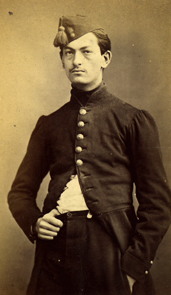
\includegraphics[width=\linewidth]{images/book3/b1-michel-levy.jpg}

{\scriptsize Michel-Lévy de estudiante, hacia 1862. Dominio público.}
\end{minipage}
\end{history}

Dos ondas que salen de un grano pueden recibir un \omterm{def:b1:optical-mineralogy:retardation}{retardo} adicional, conocido, mediante una lámina auxiliar insertada por
encima de la sección a \ang{45} de los polarizadores. La más común está cortada para mostrar el rojo de primer \omterm{def:b1:optical-mineralogy:interference-colour}{orden}, un
\omterm{def:b1:optical-mineralogy:retardation}{retardo} de unos \qty{540}{nm}. Si la dirección de vibración lenta del grano es paralela a la dirección lenta de la lámina,
los \omterm{def:b1:optical-mineralogy:retardation}{retardos} se suman y el color del grano sube en un \omterm{def:b1:optical-mineralogy:interference-colour}{orden} aproximadamente; si es paralela a la dirección rápida, se restan
y el color baja. Un grano gris de primer \omterm{def:b1:optical-mineralogy:interference-colour}{orden} de \qty{100}{nm} pasa a azul de segundo \omterm{def:b1:optical-mineralogy:interference-colour}{orden} (\qty{640}{nm}) en una
orientación y a naranja de primer \omterm{def:b1:optical-mineralogy:interference-colour}{orden} (\qty{440}{nm}) en la otra; la prueba muestra cuál de las dos direcciones de
vibración del grano es la lenta, una propiedad que sirve para identificar \omterm{def:b1:rock-forming-minerals:mineral}{minerales} alargados.

\section{Identificar minerales en lámina delgada}

\begin{definition}[Macla, macla polisintética]\label{def:b1:optical-mineralogy:twin}
Un \emph{macla}\index{macla (de cristal)} es un crecimiento de dos o más cristales del mismo \omterm{def:b1:rock-forming-minerals:mineral}{mineral} cuyas redes están
relacionadas por una simetría que el cristal por sí mismo no tiene, como una reflexión a través de un plano (el plano de
macla). La \emph{macla polisintética}\index{macla polisintética} es una macla repetida en planos paralelos, que divide un
cristal en \omterm{def:b1:field-lab-methods-1:thin-section}{láminas delgadas} y paralelas cuyas orientaciones se alternan.
\end{definition}

Entre \omterm{def:b1:field-lab-methods-1:microscope}{nicoles cruzados} las láminas de una \omterm{def:b1:optical-mineralogy:twin}{macla polisintética} se extinguen alternativamente: la mitad de ellas están oscuras
cuando la otra mitad está brillante, y el cristal parece rayado. Las \omterm{def:b1:rock-forming-minerals:groups}{plagioclasas} casi siempre muestran estas rayas, que las
distinguen de inmediato del cuarzo y del \omterm{def:b1:rock-forming-minerals:groups}{feldespato alcalino}; su otro rasgo, el \omterm{def:b1:optical-mineralogy:relief}{relieve} bajo y los colores grises a blancos de
primer \omterm{def:b1:optical-mineralogy:interference-colour}{orden}, lo comparten con ellos. Los \omterm{def:b1:optical-mineralogy:extinction}{ángulos de extinción} de los dos conjuntos de láminas, medidos a uno y otro lado del
plano de \omterm{def:b1:optical-mineralogy:twin}{macla}, dependen de la composición de la \omterm{def:b1:rock-forming-minerals:groups}{plagioclasa}, y los diagramas de esos ángulos dan su contenido en anortita.

\begin{method}[Identificar un mineral en lámina delgada]\label{met:b1:optical-mineralogy:identify}
\begin{enumerate}
  \item En \omterm{def:b1:field-lab-methods-1:microscope}{luz polarizada plana}: anótese si el grano es opaco; su color y su \omterm{def:b1:optical-mineralogy:pleochroism}{pleocroísmo} (gírese la platina); su \omterm{def:b1:optical-mineralogy:relief}{relieve}, y a
        qué lado de $1.54$ está su índice (\omterm{def:b1:optical-mineralogy:relief}{línea de Becke}); su forma y sus exfoliaciones, y el ángulo entre dos exfoliaciones.
  \item Entre \omterm{def:b1:field-lab-methods-1:microscope}{nicoles cruzados}: compruébese si permanece oscuro (isótropo, o una sección perpendicular a un \omterm{def:b1:optical-mineralogy:optic-axis}{eje óptico});
        entre los granos del mismo \omterm{def:b1:rock-forming-minerals:mineral}{mineral}, búsquese el \omterm{def:b1:optical-mineralogy:interference-colour}{color de interferencia} más alto y léase la \omterm{def:b1:optical-mineralogy:birefringence}{birrefringencia} en el \omterm{def:b1:optical-mineralogy:interference-colour}{diagrama
        de Michel-Lévy} para el espesor de la sección.
  \item Mídase el \omterm{def:b1:optical-mineralogy:extinction}{ángulo de extinción} en granos que muestren una exfoliación o un alargamiento; búsquense las \omterm{def:b1:optical-mineralogy:twin}{maclas} (rayas
        polisintéticas, \omterm{def:b1:optical-mineralogy:twin}{maclas} simples).
  \item Compárese con una tabla de propiedades ópticas (\cref{tab:b1:optical-mineralogy:key}) y con los \omterm{def:b1:rock-forming-minerals:mineral}{minerales} que la roca
        puede contener (\cref{ch:b1:rock-forming-minerals}).
\end{enumerate}
\end{method}

\begin{table}[htbp]
\centering\footnotesize
\setlength{\tabcolsep}{3pt}
% ledger: hom:quartz-optics, hom:orthoclase-optics, hom:albite-optics, hom:anorthite-optics, hom:muscovite-optics, hom:biotite-optics, hom:hornblende-optics, hom:diopside-optics, hom:forsterite-optics, hom:fayalite-optics, hom:almandine-optics, hom:calcite-optics, hom:magnetite-optics
\begin{tabular}{@{}>{\raggedright\arraybackslash}p{2.0cm}>{\raggedright\arraybackslash}p{2.6cm}>{\raggedright\arraybackslash}p{2.3cm}>{\raggedright\arraybackslash}p{1.8cm}>{\raggedright\arraybackslash}p{3.0cm}>{\raggedright\arraybackslash}p{3.8cm}@{}}
\hline
\omterm{def:b1:rock-forming-minerals:mineral}{mineral} & color (LPP) & índices & birre\-frin\-gen\-cia & color más alto a \qty{30}{\micro m} & otros rasgos \\
\hline
cuarzo & incoloro & 1.544--1.553 & 0.009 & blanco de primer \omterm{def:b1:optical-mineralogy:interference-colour}{orden} & sin exfoliación; sin \omterm{def:b1:optical-mineralogy:twin}{maclas} visibles; \omterm{def:b1:optical-mineralogy:optic-axis}{uniáxico} \\
ortoclasa & incolora, a menudo turbia & 1.518--1.525 & 0.005 & gris de primer \omterm{def:b1:optical-mineralogy:interference-colour}{orden} & \omterm{def:b1:optical-mineralogy:relief}{relieve} negativo; \omterm{def:b1:optical-mineralogy:twin}{maclas} simples \\
\omterm{def:b1:rock-forming-minerals:groups}{plagioclasa} & incolora & 1.526--1.590 & 0.008--0.013 & blanco a amarillo pálido de primer \omterm{def:b1:optical-mineralogy:interference-colour}{orden} & \omterm{def:b1:optical-mineralogy:twin}{macla polisintética} \\
moscovita & incolora & 1.552--1.618 & 0.035--0.042 & brillante, de segundo a tercer \omterm{def:b1:optical-mineralogy:interference-colour}{orden} & una exfoliación perfecta; extinción recta \\
biotita & parda, verde & 1.565--1.696 & 0.04--0.07 & enmascarado por su propio color & fuerte \omterm{def:b1:optical-mineralogy:pleochroism}{pleocroísmo}; una exfoliación perfecta \\
hornblenda & verde, parda & 1.675--1.695 & 0.020 & azul de segundo \omterm{def:b1:optical-mineralogy:interference-colour}{orden} & pleocroica; exfoliaciones a \ang{56}/\ang{124}; extinción \ang{15}--\ang{19} \\
diópsido & incoloro & 1.664--1.694 & 0.030 & amarillo de segundo \omterm{def:b1:optical-mineralogy:interference-colour}{orden} & exfoliaciones a unos \ang{87}/\ang{93}; extinción de unos \ang{38} \\
\omterm{def:b1:rock-forming-minerals:groups}{olivino} & incoloro (Mg) a amarillo pálido (Fe) & 1.635--1.879 & 0.035--0.052 & del final del segundo \omterm{def:b1:optical-mineralogy:interference-colour}{orden} al tercero & \omterm{def:b1:optical-mineralogy:relief}{relieve} alto; grietas irregulares, sin exfoliación buena \\
\omterm{def:b1:rock-forming-minerals:groups}{granate} & incoloro a rosa pálido & 1.830 (almandino) & isótropo & negro & \omterm{def:b1:optical-mineralogy:relief}{relieve} muy alto; contornos de seis u ocho lados \\
calcita & incolora & 1.486--1.658 & 0.172 & blanco de \omterm{def:b1:optical-mineralogy:interference-colour}{orden} alto & el \omterm{def:b1:optical-mineralogy:relief}{relieve} cambia al girar; exfoliación romboédrica \\
magnetita & opaca & --- & --- & --- & negra en ambas luces \\
\hline
\end{tabular}
\caption{Propiedades ópticas de \omterm{def:b1:rock-forming-minerals:mineral}{minerales} formadores de rocas comunes en \omterm{def:b1:field-lab-methods-1:thin-section}{lámina delgada}.
LPP: \omterm{def:b1:field-lab-methods-1:microscope}{luz polarizada plana}. El color más alto se lee en el \omterm{def:b1:optical-mineralogy:interference-colour}{diagrama de Michel-Lévy} en $\Delta = \qty{30000}{nm}\times\delta$.}
\label{tab:b1:optical-mineralogy:key}
\end{table}

\begin{omfigure}
\setlength{\tabcolsep}{2pt}
\begin{tabular}{cc}
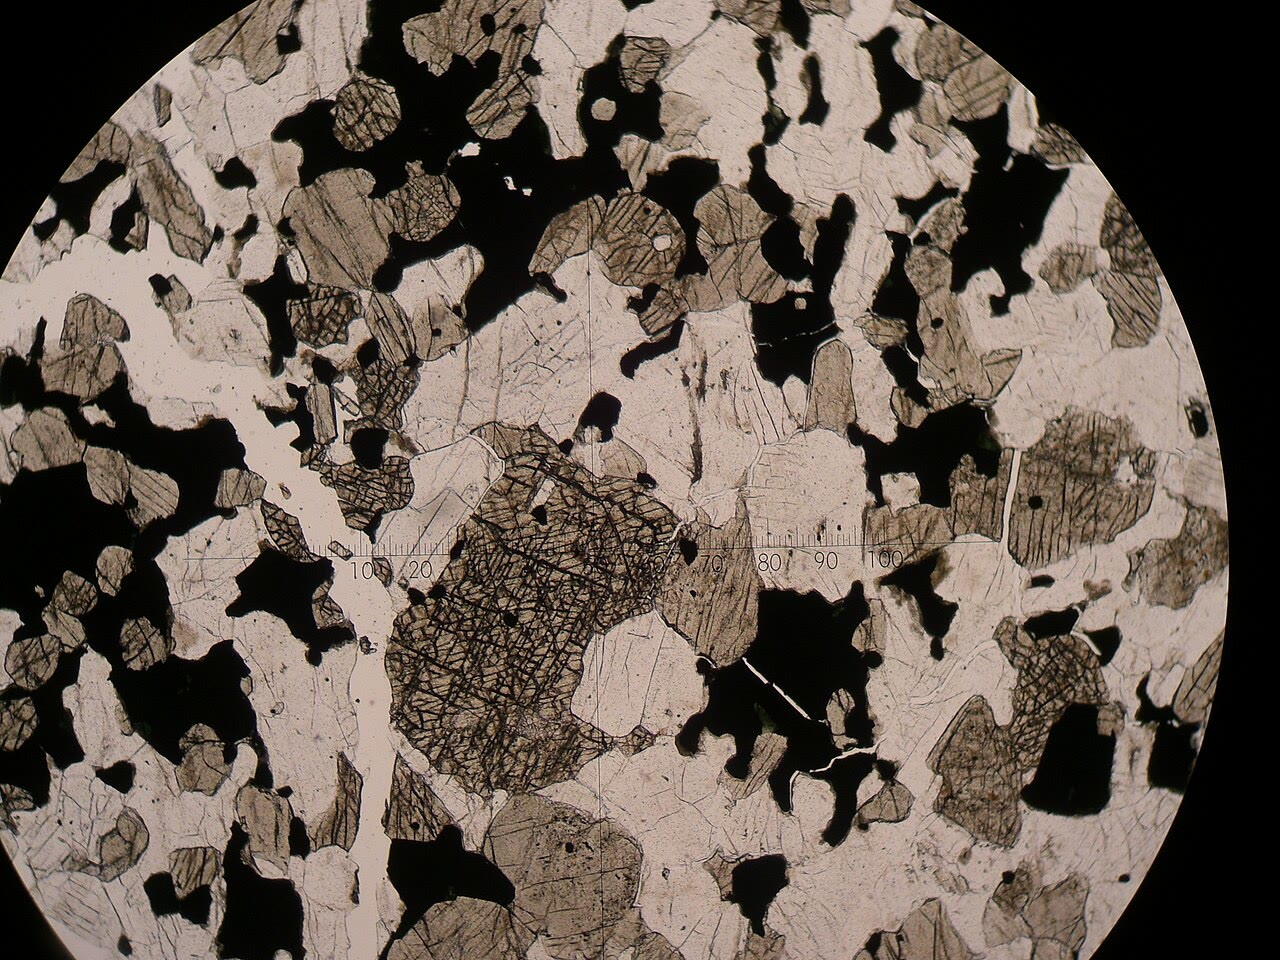
\includegraphics[width=0.485\linewidth]{images/book3/b1-gabbro-ppl.jpg} &
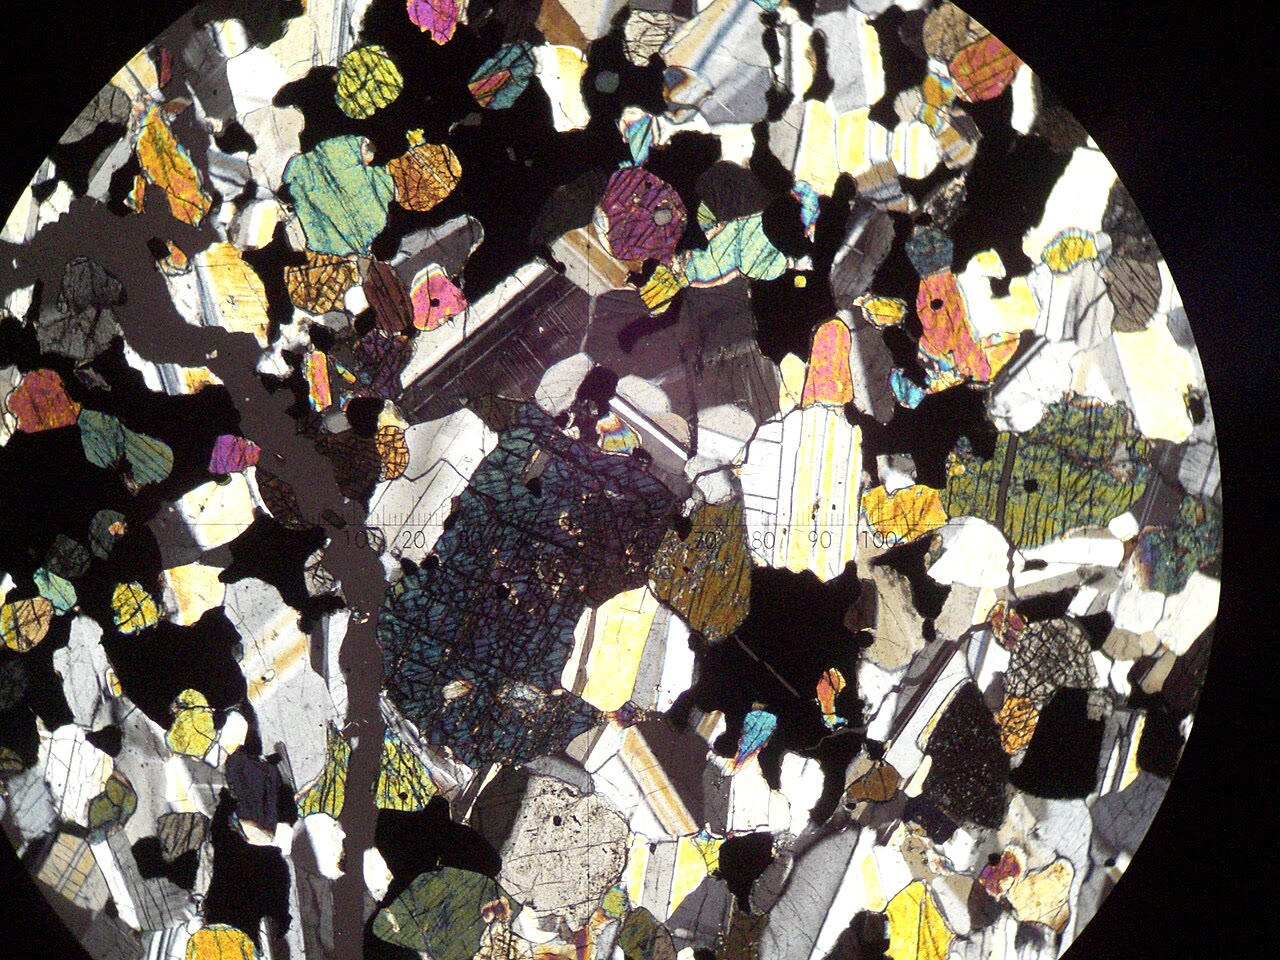
\includegraphics[width=0.485\linewidth]{images/book3/b1-gabbro-xpl.jpg} \\
{\small (a) \omterm{def:b1:field-lab-methods-1:microscope}{luz polarizada plana}} & {\small (b) \omterm{def:b1:field-lab-methods-1:microscope}{nicoles cruzados}} \\
\end{tabular}
% ledger: commons:gabbro-ppl, commons:gabbro-xpl

\medskip
{\small La misma zona de un gabro en \omterm{def:b1:field-lab-methods-1:thin-section}{lámina delgada}. En \omterm{def:b1:field-lab-methods-1:microscope}{luz polarizada plana} (a), la \omterm{def:b1:rock-forming-minerals:groups}{plagioclasa} es incolora de \omterm{def:b1:optical-mineralogy:relief}{relieve} bajo,
los granos de \omterm{def:b1:rock-forming-minerals:groups}{piroxeno} y \omterm{def:b1:rock-forming-minerals:groups}{olivino} son gris pardo pálidos de \omterm{def:b1:optical-mineralogy:relief}{relieve} alto y con grietas densas, y el \omterm{def:b1:rock-forming-minerals:mineral}{mineral} opaco es negro; la
escala es un micrómetro en el ocular. Entre \omterm{def:b1:field-lab-methods-1:microscope}{nicoles cruzados} (b), las tablillas de \omterm{def:b1:rock-forming-minerals:groups}{plagioclasa} están rayadas por la \omterm{def:b1:optical-mineralogy:twin}{macla
polisintética}, los granos de \omterm{def:b1:rock-forming-minerals:groups}{piroxeno} y \omterm{def:b1:rock-forming-minerals:groups}{olivino} brillan en colores de segundo \omterm{def:b1:optical-mineralogy:interference-colour}{orden}, y el \omterm{def:b1:rock-forming-minerals:mineral}{mineral} opaco permanece negro.
Fotografías Chmee2, CC BY-SA 3.0 (Wikimedia Commons).}
\end{omfigure}

\begin{inthelab}[Una sesión ante el microscopio]
\begin{minipage}[t]{0.55\linewidth}\vspace{0pt}
Una petróloga que describe una \omterm{def:b1:field-lab-methods-1:thin-section}{lámina delgada} nueva la recorre primero con poco aumento, para ver la textura y los \omterm{def:b1:rock-forming-minerals:mineral}{minerales}
principales, y después grano a grano. Para cada \omterm{def:b1:rock-forming-minerals:mineral}{mineral} anota las observaciones del método anterior, estima su proporción en
el campo y registra cómo se tocan los granos: cuál cristalizó primero, cuáles rellenan los huecos que quedan, cuáles
reemplazan a otros. Las medidas ópticas se hacen con la platina graduada en grados y una lámina auxiliar; las composiciones,
cuando importan, se miden después con una microsonda sobre la misma sección. Un laboratorio docente funciona de la misma
manera, con un microscopio por estudiante y una caja de láminas de referencia de \omterm{def:b1:rock-forming-minerals:mineral}{minerales} conocidos junto a él.
\end{minipage}\hfill
\begin{minipage}[t]{0.42\linewidth}\vspace{0pt}
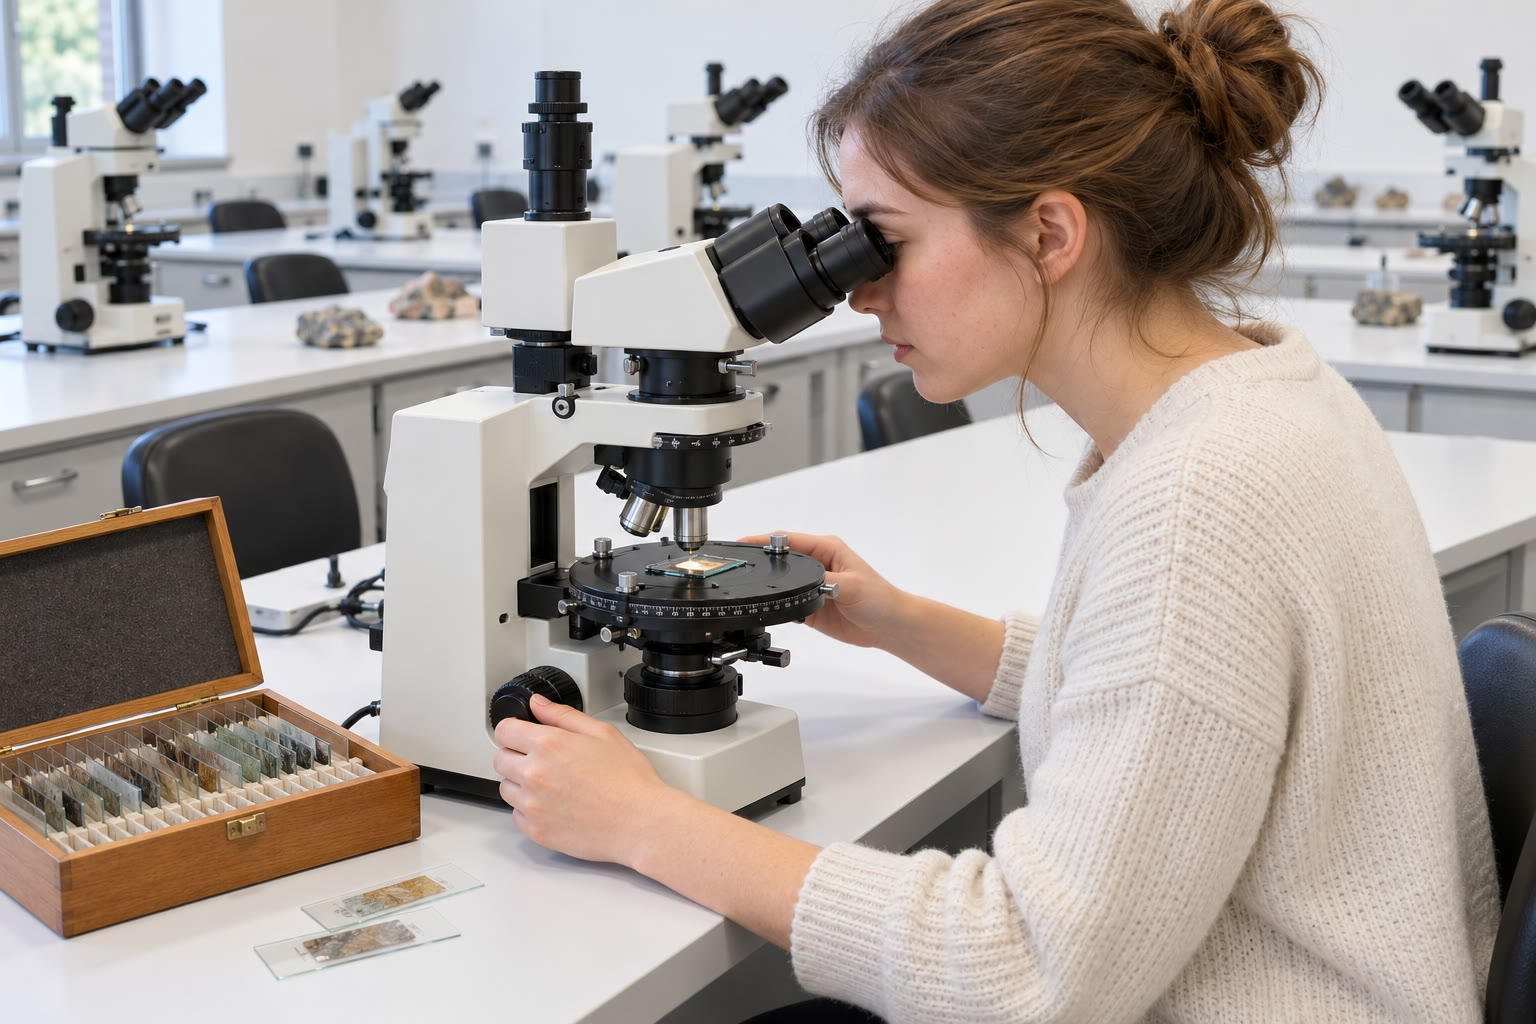
\includegraphics[width=\linewidth]{images/book3/ai/b1-microscope-student.jpg}

{\scriptsize Un estudiante ante un \omterm{def:b1:field-lab-methods-1:microscope}{microscopio de polarización} en un laboratorio docente (ilustración generada por IA).}
\end{minipage}
\end{inthelab}

\section{Ejercicios}

\begin{exercise}[$\star$]\label{exo:b1:optical-mineralogy:1}
Calcúlese el mayor \omterm{def:b1:optical-mineralogy:retardation}{retardo} del cuarzo ($\delta = 0.009$) y el de la calcita ($\delta = 0.172$) en una sección de
\qty{30}{\micro m} de espesor. Con el \omterm{def:b1:optical-mineralogy:interference-colour}{diagrama de Michel-Lévy}, descríbase el color de cada uno.
% ledger: hom:quartz-optics, hom:calcite-optics
\end{exercise}

\begin{exercise}[$\star$]\label{exo:b1:optical-mineralogy:2}
Un grano se gira en la platina entre \omterm{def:b1:field-lab-methods-1:microscope}{nicoles cruzados}. Calcúlese $I/I_0$, como fracción de su máximo, en $\theta = 0$,
\ang{22.5}, \ang{45}, \ang{67.5} y \ang{90} a partir de una \omterm{def:b1:optical-mineralogy:extinction}{posición de extinción}.
\end{exercise}

\begin{exercise}[$\star$]\label{exo:b1:optical-mineralogy:3}
Explíquese por qué un \omterm{def:b1:rock-forming-minerals:groups}{granate} permanece negro entre \omterm{def:b1:field-lab-methods-1:microscope}{nicoles cruzados} cualquiera que sea la posición de la platina, y por qué
un grano de cuarzo puede hacer lo mismo. ¿Cómo se distinguirían en \omterm{def:b1:field-lab-methods-1:microscope}{luz polarizada plana}?
\end{exercise}

\begin{exercise}[$\star$]\label{exo:b1:optical-mineralogy:4}
Ordénense por \omterm{def:b1:optical-mineralogy:relief}{relieve}, en un medio de índice $1.54$, la ortoclasa ($n$ hacia $1.52$), el cuarzo ($1.55$), la forsterita
($1.65$) y el almandino ($1.83$). ¿Cuál tiene \omterm{def:b1:optical-mineralogy:relief}{relieve} negativo? ¿En qué dirección se mueve su \omterm{def:b1:optical-mineralogy:relief}{línea de Becke} al subir el foco?
% ledger: hom:orthoclase-optics, hom:quartz-optics, hom:forsterite-optics, hom:almandine-optics
\end{exercise}

\begin{exercise}[$\star\star$]\label{exo:b1:optical-mineralogy:5}
En una sección de \qty{30}{\micro m}, los granos de un \omterm{def:b1:rock-forming-minerals:mineral}{mineral} verde \omterm{def:b1:optical-mineralogy:pleochroism}{pleocroico} con dos exfoliaciones a \ang{56} y \ang{124}
muestran a lo sumo un azul de segundo \omterm{def:b1:optical-mineralogy:interference-colour}{orden}, leído en el diagrama como $\Delta = \qty{650}{nm}$. Calcúlese su
\omterm{def:b1:optical-mineralogy:birefringence}{birrefringencia} y nómbrese el \omterm{def:b1:rock-forming-minerals:mineral}{mineral} con \cref{tab:b1:optical-mineralogy:key}.
\end{exercise}

\begin{exercise}[$\star\star$]\label{exo:b1:optical-mineralogy:6}
Con \cref{prop:b1:optical-mineralogy:relief} con $n_m = 1.54$ e $i = \ang{30}$, calcúlese la desviación en el borde de un
grano de cuarzo ($n = 1.553$) y de uno de forsterita ($n = 1.651$), en grados, y el cociente entre ambas. Compruébese la
segunda con la ley de Snell exacta.
\end{exercise}

\begin{exercise}[$\star\star$]\label{exo:b1:optical-mineralogy:7}
Una lámina roja de primer \omterm{def:b1:optical-mineralogy:interference-colour}{orden} tiene $\Delta = \qty{540}{nm}$. Un grano de cuarzo de $\Delta = \qty{270}{nm}$ se coloca a
\ang{45} con la lámina insertada. ¿Cuáles son los dos \omterm{def:b1:optical-mineralogy:retardation}{retardos} totales posibles, y los colores que dan en el diagrama?
¿Qué orientación pone las dos direcciones lentas paralelas?
\end{exercise}

\begin{exercise}[$\star\star$]\label{exo:b1:optical-mineralogy:8}
En su borde afilado, un grano de fayalita ($\delta = 0.052$) adelgaza desde \qty{30}{\micro m} hasta cero. ¿Cuántos matices
rojo violáceos, que terminan los órdenes en 542, 1074 y \qty{1605}{nm}, aparecen como franjas de color entre el borde y la
parte de espesor completo del grano?
% ledger: hom:fayalite-optics
\end{exercise}

\begin{exercise}[$\star\star$]\label{exo:b1:optical-mineralogy:9}
En varios granos alargados con una exfoliación buena, un geólogo mide \omterm{def:b1:optical-mineralogy:extinction}{ángulos de extinción} de \ang{0}, \ang{21}, \ang{36} y
\ang{37} entre la traza de exfoliación y la dirección de vibración lenta. ¿Por qué difieren los valores? ¿Es más probable
que el \omterm{def:b1:rock-forming-minerals:mineral}{mineral} sea diópsido u hornblenda?
% ledger: hom:diopside-optics, hom:hornblende-optics
\end{exercise}

\begin{exercise}[$\star\star\star$]\label{exo:b1:optical-mineralogy:10}
Rehágase la demostración de \cref{thm:b1:optical-mineralogy:intensity} con el analizador paralelo al polarizador, y muéstrese que
$I_\parallel = I_0\bigl(1 - \sin^2 2\theta\sin^2(\pi\Delta/\lambda)\bigr)$. ¿Qué color muestra un grano de $\Delta = \qty{550}{nm}$
a \ang{45} entre polarizadores paralelos?
\end{exercise}

\begin{exercise}[$\star\star\star$]\label{exo:b1:optical-mineralogy:11}
Para un grano de calcita con $\Delta = \qty{5000}{nm}$, el factor $\sin^2(\pi\Delta/\lambda)$ se anula siempre que $\Delta/\lambda$
es un número entero. (a) ¿Cuántas veces se anula entre \num{400} y \qty{700}{nm}? (b) Muéstrese que cerca de
$\lambda = \qty{550}{nm}$ dos ceros sucesivos están separados unos $\lambda^2/\Delta$, y calcúlese. (c) Explíquese por qué
el grano parece casi blanco.
\end{exercise}

\begin{exercise}[$\star\star\star$]\label{exo:b1:optical-mineralogy:12}
Muéstrese que, promediado sobre una vuelta completa de la platina, un grano entre \omterm{def:b1:field-lab-methods-1:microscope}{nicoles cruzados} deja pasar
$\frac12 I_0\sin^2(\pi\Delta/\lambda)$. Una geóloga estima \omterm{def:b1:optical-mineralogy:birefringence}{birrefringencias} a partir del color más alto de cada \omterm{def:b1:rock-forming-minerals:mineral}{mineral},
suponiendo \qty{30}{\micro m}, en una sección que en realidad tiene \qty{25}{\micro m} de espesor. ¿Por qué factor están
equivocados todos sus valores, y en qué sentido?
\end{exercise}

\section{Problema: identificar los minerales de una lámina desconocida}

\begin{problem}[{Problema de fin de semana --- observar el relieve, el pleocroísmo y los colores de interferencia, medir el
espesor de una sección con cuarzo y nombrar sus minerales}]
\label{pb:b1:optical-mineralogy:1}
% values: calc/ch08.py; optical data: ledger hom:*-optics
% ledger: hom:quartz-optics, hom:diopside-optics, hom:forsterite-optics, hom:albite-optics, hom:anorthite-optics, hom:hornblende-optics, hom:biotite-optics
Una \omterm{def:b1:field-lab-methods-1:thin-section}{lámina delgada} de una roca ígnea desconocida, montada en una resina de índice $1.540$, tiene, según se dice,
\qty{30}{\micro m} de espesor. Contiene cinco \omterm{def:b1:rock-forming-minerals:mineral}{minerales}, designados de A a E. Úsense la tabla de propiedades ópticas del
capítulo, el \omterm{def:b1:optical-mineralogy:interference-colour}{diagrama de Michel-Lévy} y los valores siguientes: cuarzo $n_\omega = 1.544$, $n_\varepsilon = 1.553$; diópsido
$n_\alpha = 1.664$, $n_\beta = 1.672$, $n_\gamma = 1.694$.

\medskip
\noindent\textbf{Parte I --- Luz polarizada plana.}
\begin{enumerate}
  \item El \omterm{def:b1:rock-forming-minerals:mineral}{mineral} A es incoloro, con bordes de grano difíciles de ver. El \omterm{def:b1:rock-forming-minerals:mineral}{mineral} B es incoloro, con bordes oscuros
        marcados y dos exfoliaciones que se cortan hacia \ang{87}. ¿Cuál tiene mayor \omterm{def:b1:optical-mineralogy:relief}{relieve}?
  \item Para A, tomado como cuarzo, y B, tomado como diópsido, calcúlese $|n - n_m|$ usando la media de los índices
        principales de cada uno.
  \item Con \cref{prop:b1:optical-mineralogy:relief}, calcúlese el cociente de las desviaciones en sus bordes para la misma
        inclinación de la frontera.
  \item Al subir el foco, la \omterm{def:b1:optical-mineralogy:relief}{línea de Becke} de B entra en el grano. ¿Qué indica esto?
  \item El \omterm{def:b1:rock-forming-minerals:mineral}{mineral} C pasa de amarillo pálido a pardo oscuro al girar la platina, más oscuro cuando su única exfoliación
        está según el polarizador. Nómbrese la propiedad y el \omterm{def:b1:rock-forming-minerals:mineral}{mineral}.
  \item El \omterm{def:b1:rock-forming-minerals:mineral}{mineral} D es incoloro, de \omterm{def:b1:optical-mineralogy:relief}{relieve} bajo, en tablillas largas; E es verde a amarillo y \omterm{def:b1:optical-mineralogy:pleochroism}{pleocroico}, con dos
        exfoliaciones a \ang{124}. ¿Qué sugiere el ángulo para E?
\end{enumerate}

\medskip
\noindent\textbf{Parte II --- El espesor de la sección.}
\begin{enumerate}[resume]
  \item ¿Cuál es el mayor \omterm{def:b1:optical-mineralogy:retardation}{retardo} del cuarzo en una sección de exactamente \qty{30}{\micro m}? ¿Qué color tiene?
  \item ¿Por qué hay que buscar el mayor \omterm{def:b1:optical-mineralogy:retardation}{retardo} entre muchos granos de A, en lugar de medirlo en uno cualquiera?
  \item El color más alto que muestran los granos de A es un amarillo pálido de primer \omterm{def:b1:optical-mineralogy:interference-colour}{orden}; un comparador de cuña de cuarzo
        da su \omterm{def:b1:optical-mineralogy:retardation}{retardo} como \qty{342}{nm}. Calcúlese el espesor real de la sección.
  \item ¿En qué porcentaje es la sección más gruesa de lo que debería ser?
  \item A $\lambda = \qty{550}{nm}$ y \ang{45} de la extinción, calcúlese $I/I_0$ para este grano de cuarzo, y para el mismo
        grano en una sección de \qty{30}{\micro m}.
  \item Calcúlese el intervalo de \omterm{def:b1:optical-mineralogy:retardation}{retardos} de D, tomado como \omterm{def:b1:rock-forming-minerals:groups}{plagioclasa} ($\delta = 0.008$ a $0.013$), en esta sección, y
        dígase si sus colores permanecen en el primer \omterm{def:b1:optical-mineralogy:interference-colour}{orden}.
\end{enumerate}

\medskip
\noindent\textbf{Parte III --- La birrefringencia de B.}
\begin{enumerate}[resume]
  \item El color más alto de B es un azul que se lee como $\Delta = \qty{1140}{nm}$. ¿En qué \omterm{def:b1:optical-mineralogy:interference-colour}{orden} está?
  \item Calcúlese la \omterm{def:b1:optical-mineralogy:birefringence}{birrefringencia} de B con el espesor hallado en la pregunta 9.
  \item ¿Qué \omterm{def:b1:optical-mineralogy:birefringence}{birrefringencia} se habría hallado suponiendo \qty{30}{\micro m}? ¿Qué \omterm{def:b1:rock-forming-minerals:mineral}{mineral} incoloro de \omterm{def:b1:optical-mineralogy:relief}{relieve} alto habría
        sugerido, y por qué está fuera de lugar en una roca con cuarzo (considérese \ce{Mg2SiO4 + SiO2 -> 2 MgSiO3})?
  \item Compárese el resultado de la pregunta 14 con la tabla, junto con el \omterm{def:b1:optical-mineralogy:relief}{relieve} y las exfoliaciones de B, y concluya.
  \item ¿Qué color mostraría B como mucho en una sección correcta de \qty{30}{\micro m}?
  \item La sección se desbasta hasta \qty{30}{\micro m}. ¿Cuánto hay que adelgazarla, y cuál es entonces el color más alto del cuarzo?
\end{enumerate}

\medskip
\noindent\textbf{Parte IV --- Extinción y maclado.}
\begin{enumerate}[resume]
  \item Las tablillas de D están divididas en franjas paralelas que se extinguen alternativamente. Nómbrese el rasgo y el \omterm{def:b1:rock-forming-minerals:mineral}{mineral}.
  \item Las franjas de una tablilla se extinguen a \ang{27} y \ang{28} a uno y otro lado del plano de \omterm{def:b1:optical-mineralogy:twin}{macla}. ¿Qué dan esos
        ángulos, medidos en muchas tablillas, al compararlos con diagramas publicados?
  \item El mayor \omterm{def:b1:optical-mineralogy:extinction}{ángulo de extinción} entre las exfoliaciones de E y su dirección lenta es \ang{17}. Nombre E.
  \item Calcúlese el mayor \omterm{def:b1:optical-mineralogy:retardation}{retardo} de E en esta sección y el color que muestra.
  \item Un grano de B permanece oscuro durante una vuelta completa. Explíquese cómo puede ser el mismo \omterm{def:b1:rock-forming-minerals:mineral}{mineral} que los granos
        brillantes de B.
  \item Enumérense los \omterm{def:b1:rock-forming-minerals:mineral}{minerales} de A a E, y dígase qué tipo de roca forman.
  \item ¿Cuál es el espesor real de la sección, en micrómetros?
\end{enumerate}
\end{problem}
